\documentclass{article}

% use Times
\usepackage{times}
% For figures
\usepackage{graphicx} % more modern
%\usepackage{epsfig} % less modern
\usepackage{subfigure} 

% For citations
\usepackage{natbib}

% For algorithms
\usepackage{algorithm}
\usepackage{algorithmic}

% As of 2011, we use the hyperref package to produce hyperlinks in the
% resulting PDF.  If this breaks your system, please commend out the
% following usepackage line and replace \usepackage{icml2015} with
% \usepackage[nohyperref]{icml2015} above.
\usepackage{cleveref}
\usepackage{hyperref}

% Packages hyperref and algorithmic misbehave sometimes.  We can fix
% this with the following command.
\newcommand{\theHalgorithm}{\arabic{algorithm}}

% Employ the following version of the ``usepackage'' statement for
% submitting the draft version of the paper for review.  This will set
% the note in the first column to ``Under review.  Do not distribute.''
\usepackage{icml2015stylefiles/icml2015} 

% Employ this version of the ``usepackage'' statement after the paper has
% been accepted, when creating the final version.  This will set the
% note in the first column to ``Proceedings of the...''
%\usepackage[accepted]{icml2015}

\usepackage{tikz}
\usepackage{dsfont}
\usepackage{amsmath}
\usepackage{amssymb}
\usepackage{amsthm}


\setlength{\marginparwidth}{10ex}%added by Yifan so that the todos can fit in the margin
%\usepackage[obeyFinal]{todonotes}
\usepackage{todonotes}

\newcommand{\tinytodo}[2][]{\todo[size=\tiny]{#2}}
%\newcommand{\tinytodo}[2][]{\todo[size=\tiny, #1]{\begin{spacing}{1.0}#2\end{spacing}}}
\newcommand{\todot}[2][]{\tinytodo[color=blue!20, #1]{T: #2}} % Tor
\newcommand{\todof}[2][]{\tinytodo[color=red!20, #1]{F:\@#2}} % Finn
\newcommand{\todom}[2][]{\tinytodo[color=green!20, #1]{M:\@#2}} % Mark


\graphicspath{ {figures/} }
\usetikzlibrary{arrows,positioning} 
\tikzset{
    %Define standard arrow tip
    >=stealth',
    %Define style for boxes
    observed/.style={
           circle,
           rounded corners,
           draw=black, thick,
           minimum width=2.5em,
           minimum height=2.5em,
           font=\footnotesize,
           text centered,
           fill=blue!20!white},
     latent/.style={
           circle,
           rounded corners,
           draw=black, thick, dashed,
           minimum width=.5em,
           minimum height=.5em,
           font=\footnotesize,
           text centered,
           fill=black!10!white
           },
     empty/.style={
           circle,
           rounded corners,
           minimum width=.5em,
           minimum height=.5em,
           font=\footnotesize,
           text centered,
           },
    % Define arrow style
    pil/.style={
           o->,
           thick,
           shorten <=2pt,
           shorten >=2pt,},
    sh/.style={ shade, shading=axis, left color=red, right color=green,
    shading angle=45 }  
}

\newcommand{\defined}{\vcentcolon =}
\newcommand{\rdefined}{=\vcentcolon}
\newcommand{\E}[1]{\mathbb E\left[#1\right]}
\newcommand{\R}{\mathbb R}
\newcommand{\Var}{\operatorname{Var}}
\newcommand{\calF}{\mathcal F}
\newcommand{\sr}[1]{\stackrel{#1}}
\newcommand{\set}[1]{\left\{#1\right\}}
\newcommand{\ind}[1]{\mathds{1}\!\!\set{#1}}
\newcommand{\argmax}{\operatornamewithlimits{arg\,max}}
\newcommand{\argmin}{\operatornamewithlimits{arg\,min}}
\newcommand{\floor}[1]{\left \lfloor {#1} \right\rfloor}
\newcommand{\ceil}[1]{\left \lceil {#1} \right\rceil}
\newcommand{\eqn}[1]{\begin{align}#1\end{align}}
\newcommand{\eq}[1]{\begin{align*}#1\end{align*}}
\newcommand{\Ber}{\operatorname{Bernoulli}}
\renewcommand{\P}[1]{\operatorname{P}\left\{#1\right\}}
\newcommand{\Pri}[1]{\operatorname{P}_i\left\{#1\right\}}
\newcommand{\Prz}[1]{\operatorname{P}_0\left\{#1\right\}}
\newcommand{\bigo}[1]{\mathcal{O}\left( #1 \right)}
\newcommand{\bigotilde}[1]{\tilde{\mathcal{O}}\left( #1 \right)}
\newcommand{\bigtheta}[1]{\Theta\left( #1 \right)}
\newcommand{\bigthetatilde}[1]{\tilde{\Theta}\left( #1 \right)}
\newcommand{\bigomega}[1]{\Omega\left( #1 \right)}
\newcommand{\KL}{\operatorname{KL}}

\newcommand{\etc}{\textit{etc}}
\newcommand{\ie}{\textit{i.e.}}
\newcommand{\eg}{\textit{e.g.}}

\theoremstyle{plain}
\newtheorem{theorem}{Theorem}
\newtheorem{proposition}[theorem]{Proposition}
\newtheorem{lemma}[theorem]{Lemma}
\newtheorem{corollary}[theorem]{Corollary}
\theoremstyle{definition}
\newtheorem{definition}[theorem]{Definition}
\newtheorem{assumption}[theorem]{Assumption}
\newtheorem{remark}[theorem]{Remark}
\newtheorem{example}[theorem]{Example}

% The \icmltitle you define below is probably too long as a header.
% Therefore, a short form for the running title is supplied here:
\icmltitlerunning{Causal Bandits}

\begin{document} 

\twocolumn[
\icmltitle{Casual Bandits}

% It is OKAY to include author information, even for blind
% submissions: the style file will automatically remove it for you
% unless you've provided the [accepted] option to the icml2015
% package.
\icmlauthor{Your Name}{email@yourdomain.edu}
\icmladdress{Your Fantastic Institute,
            314159 Pi St., Palo Alto, CA 94306 USA}
\icmlauthor{Your CoAuthor's Name}{email@coauthordomain.edu}
\icmladdress{Their Fantastic Institute,
            27182 Exp St., Toronto, ON M6H 2T1 CANADA}

% You may provide any keywords that you 
% find helpful for describing your paper; these are used to populate 
% the "keywords" metadata in the PDF but will not be shown in the document
\icmlkeywords{causal,bandit}

\vskip 0.3in
]

\begin{abstract} 
We study the problem of using causal models to improve the rate at which good interventions can be learned online in a stochastic environment. 
Our formalism combines multi-arm bandits and causal inference to model a novel type of bandit feedback that is not exploited by existing approaches.
We propose a new algorithm that can make use of the causal feedback and prove that it achieves bounds on both simple and cumulative regret that are strictly better (in dependence on the number of possible interventions and number of rounds) than algorithms which do not use the additional causal information.
\end{abstract} 

%%%%%%%%%%%%%%%%%%%%%%%%%%%%%%%%%%%%%%%%%%%%%%%%%
% INTRODUCTION
%%%%%%%%%%%%%%%%%%%%%%%%%%%%%%%%%%%%%%%%%%%%%%%%%
\section{Introduction}

A classical problem in economics and operations research is how to choose interventions that maximise utility. 
We study an idealised model of such interventions using a combination of the multi-armed bandit framework \citep{Robbins1952} and the theory/language of causal inference 
\citep{Pearl2000}.

\todom{Describe feature of class of problem; highlight with examples.}

The challenge is best illustrated with an example. Consider a farmer wishing to optimise the yield of her crop. 
She knows that crop yield is only affected by temperature, a particular soil nutrient, and moisture level but the precise effect of their combination is unknown.
In each season the farmer has enough time and money to intervene and control at most one of these variables:
deploying shade or heat lamps will set the temperature to be low or high; the nutrient can be added or removed a through a choice of fertilizer; and irrigation or rain-proof covers will keep the soil wet or dry.
When not intervened upon, the temperature, soil, and moisture vary naturally from season to season due to weather conditions and these are all observed along with the final crop yield at the end of each season.
How might the farmer best experiment to identify the single, highest yielding intervention without sacrificing too much crop yield (relative to always choosing the best intervention) in the process?

One obvious approach would be to cast the above example as a stochastic multi-armed bandit problem~\cite{Robbins1952} -- each of the six possible interventions is an arm and the crop yield is the reward -- and apply an algorithm such as UCB~\cite{Auer1995} with well understood regret guarantees.
However, as we show in \S\ref{sec:results}, this approach ignores the extra information available in the non-intervened variables and subsequently yields a worst-case regret with a sub-optimal dependence on the number of possible interventions.

There has been a significant amount of recent work which proposes alternative modes of feedback within the bandit setting \cite{TODO} as well as results for partial monitoring which, as first glance, may appear applicable. As we show in Section~\ref{}, applying these results to our problem also exhibit a sub-optimal dependence on the number of available interventions.

\todom{Rework rest of intro}

%Problems requiring choosing an action under uncertainty are rife in all areas of human endeavour. For many problems, actions may be chosen sequentially, allowing the agent to learn from the outcome of early choices to improve later ones. 

% A widely used framework for sequential decision making is the multi-armed bandit. In the classic multi-armed bandit setting there is a finite set of available actions, each associated with a distribution over rewards which is unknown but stationary. At each timestep the agent selects an action and receives a reward sampled i.i.d from the corresponding reward distribution. The performance of bandit algorithms is described by the regret: the difference in the expected reward obtained by the algorithm and the reward that could be obtained if the optimal action was selected at every timestep. 

An alternate approach to selecting actions is causal inference. Frameworks for causal inference provide a mechanism to specify assumptions that allow observational distributions over variables to be mapped to interventional ones. This allows an agent to predict the outcome of an action based on non-experimental data. This approach is common in social science, demography, and economics where explicit experimentation may be difficult. For example, predicting the effect of changes to childcare subsidies on workforce participation or school choice on student grades. 

We take a first step towards unifying these approaches by considering a variant of the stochastic multi-armed bandit problem where we have prior knowledge of the causal structure governing the available actions. 

\todom{Summarise results \& give intuition for algorithm}

A natural way to connect the causal framework with the bandit setting is to model the problem as a causal directed acyclic graph. Each possible assignment of variables to values is an action (bandit arm). The reward could be a general function of the action selected and the final state of the graph. However for simplicity, we will consider the reward to be the value of a single specified node minus the cost of the selected action. The number of actions grows exponentially with the number of variables in the graph, making it important to use algorithms that take account of the graph structure to reduce the search space. 

Problems framed in this way take on characteristics of different bandit settings depending on the assumptions we make about what subset of actions can be taken, what variables are observable and whether they are observed before or after an action is selected. If feedback is received only on the reward node then the do-calculus can be applied to eliminate some actions immediately, before any experiments are performed and then a standard bandit algorithm can be run on the remaining actions. 

If we receive feedback on additional nodes the problem can be more interesting. In addition to being able to eliminate some actions prior to sampling any data as in the previous case, taking one action may give us some information on actions that were not selected. 

We consider a bandit problem where the actions and reward are represented by a specific causal graph that demonstrates this interesting structure. We develop an algorithm to leverage the information provided by this structure and demonstrate it substantially outperforms standard bandit algorithms applied to the same problem where the number of actions is large.

There has been substantial recent work into extending bandit algorithms to incorporate additional assumptions and deal with more complex feedback structures. Algorithms with strong guarantees have been developed for linear bandits [], generalized linear bandits, gaussian process bandits [], etc. There is also an active line of research into bandits with feedback defined by a graph. Actions are modelled as nodes in the graph and the agent observes rewards for each action connected to the selected action []. The novelty of our work is that we assume prior knowledge of the causal structure but not the functional form of the relationship between variables.   

Partial monitoring is a very general framework for for decoupling the feedback from the action and reward. It can be used to classify problems into one of four categories, trivial with no regret, easy with $R_T = \bigthetatilde{\sqrt{T}}$ , hard with $R_T = \bigtheta{T^{2/3}}$ and hopeless with $R_T = \bigomega{T}$ \cite{Bartok2014}. Partial monitoring algorithms yield results that are optimal with respect the horizon $T$ but not other parameters, such as $K$, which is the key focus of incorporating causal structure. 

ALSO NEED TO MENTION ANY OTHER COMBINATIONS OF BANDITS+CAUSAL (eg the Elias NIPS paper and Generalized Thompson Sampling paper)

Key to Elias' paper is: observing the action an agent would take if it were allowed to make its natural choice can provide some information about hidden confounders that influence both the reward and the choice of action. Therefore, incorporating an agents natural choice as context may outperform a standard bandit that does not use that context. (Note: even in the presence of hidden confounders, including the agents natural choice as context only may improve the results. It is easy to come up with a counter example in which it does not).

%%%%%%%%%%%%%%%%%%%%%%%%%%%%%%%%%%%%%%%%%%%%%%%%%
% PROBLEM SETUP
%%%%%%%%%%%%%%%%%%%%%%%%%%%%%%%%%%%%%%%%%%%%%%%%%
\section{Problem Setup}

\newcommand{\bernoulli}{\operatorname{Bernoulli}}
\newcommand{\dirac}{\operatorname{Dirac}}

Assume we have a known causal model with binary variables $\boldsymbol{X} = \{X_{1},\ldots,X_{N}\}$ that independently cause a 
target variable of interest $Y \in \R$ (see Figure \ref{fig:causalStructure}).
\begin{figure}[h]
\centering
\caption{Assumed Causal Structure}
\label{fig:causalStructure}
\begin{tikzpicture}[->,>=stealth',shorten >=1pt,auto,node distance=1cm,
  thick,main node/.style={observed}, hidden/.style={empty}]

 %nodes
\node[main node](1){$X_{1}$};
\node[main node, right=of 1](2){$X_{2}$};
\node[hidden, right=of 2](3){$...$};
\node[main node, right=of 3](4){$X_{N}$};
\node[main node, below right=of 2](5){Y};
 \path[every node/.style={font=\sffamily\small}]
    (1) edge (5)
    	(2) edge (5)
    (4) edge (5);
	
\end{tikzpicture}
\end{figure}


The game proceeds over $T$ identical rounds (or time-steps).
In each round $t$ the learner can choose either to do nothing or they can choose a variable $I_t \in \set{1,\ldots,N}$ and
an intervention $J_t \in \set{0,1}$. After the learner has chosen an intervention they observe $X_{t,i} \in \set{0,1}$ for all $i$ where
\eq{
X_{t,i} \sim \begin{cases}
\dirac(J_t) & \text{if } I_t = i \\
\bernoulli(q_i) & \text{otherwise}\,.
\end{cases}
}
where $\boldsymbol{q} \in [0,1]^N$ is a (possibly unknown) vector of probabilities with $q_i = \P{X_i = 1}$. Note that if the learner did not choose an intervention then $I_t$ is undefined
and $X_{t,i} \sim \bernoulli(q_i)$ for all variables $i \in \set{1,\ldots,N}$.
Finally the learner observes the reward $Y_t = r(X_t) + \eta_t$ where 
\eq{
r : \set{0,1}^N \to \R
}
is arbitrary (and unknown) 
and $\eta_t$ is a $1$-subgaussian noise
term (with the distribution possibly dependent on $X_t$). 
\todom{Connect to opening ex.}

The expected reward for intervening on variable $i$ by setting it to $j$ is defined by
\eq{
\mu_{i,j} 
&= \E{r(X)|do(X_i = j)} \\
&= \sum_{\boldsymbol{x} \in \set{0,1}^N : x_i = j} r(\boldsymbol{x})  \prod_{k \neq i} q_k^{x_k} (1 - q_k)^{1-x_k} \,. 
}
The optimal intervention is $(i^*,j^*) = \argmax_{i,j} \mu_{i,j}$ and the corresponding optimal reward is $\mu^* = \mu_{i^*,j^*}$. 
Note that the expected reward of the optimal intervention is at least as large as the expected reward for doing nothing.

It is worth mentioning that the problem may be treated as a multi-armed bandit with $2N$ arms, one corresponding to each intervention.
As we shall shortly see, this approach is usually not practical because the resulting algorithms do not exploit the structure in
the covariates.


\begin{remark}
In order to be consistent with the literature on causal inference we use the notation $do()$ to denote the action of doing nothing and $do(X_{t,I_t} = J_t)$
the action of intervening on the $I_t$th variable and setting it to equal $J_t$. 
In the bandit community it is implicit that 
algorithms selecting actions are intervening in the system. So it is sufficient to index actions according to the variable and value. 
However, in causal graphs, it is essential to differentiate observing (or conditioning) on a variable taking a certain value, from 
intervening to set that variable. Although in the specific causal graph we consider, observation and intervention are the same, we 
deliberately introduce the do-notation \cite{Pearl2000} that makes this distinction clear so as to help provide a bridge between the 
bandit and causal inference communities.
\end{remark}


We consider two standard performance measures. The first is the cumulative regret, which measures the difference between the reward expected under
the omnipotent strategy that knows the optimal action in advance and the expected reward of the learner. 
\eqn{
\label{eq:regret}
R_T = T \mu^* - \E{\sum_{t=1}^T Y_t}\,.
}
The second performance measure is the simple regret, which measures the performance of the learner on the final round only.
\eqn{
\label{eq:regret-simple}
r_T = \mu^* - \E{\mu_{I_T,J_T}}\,.
}
Both versions of the regret are useful in different circumstances. The first is most useful when the learner is truly online and can change their policy over time.
The second is useful when the exploration budget is limited and a fixed policy should eventually be chosen. \todot{make this nicer}


%%%%%%%%%%%%%%%%%%%%%%%%%%%%%%%%%%%%%%%%%%%%%%%%%
% UPPER BOUND ON SIMPLE REGRET
%%%%%%%%%%%%%%%%%%%%%%%%%%%%%%%%%%%%%%%%%%%%%%%%%
\section{Upper Bounds on the Simple Regret}

In this section we develop and analyse an algorithm for minimising the simple regret in the
causal bandit problem.  

From a causal perspective the key insight is that the assumed causal structure implies that
the law of $Y_t$ given we intervene to set $X_{t,i} = j$ is the same as the law of $Y_t$ conditioned
on $X_{t,i} = j$. Formally,
\eqn {
\label{eq:observe}
\P{Y_t \leq y|do(X_{t,i} = j)} = \P{Y_t \leq y|do(),X_{t,i} = j}\,.
}
This follows from application of the do-calculus \cite{Pearl2000} to our specific causal graph. It is not the case in general. 
For example if there was a variable $X'$ that caused both $X_{t,i}$ and $Y$ (or $X_{t,i}$ and any other variable $X_{t,l}$), 
that would introduce a backdoor path from $X_{t,i} \rightarrow Y_t$ and we would have to condition on $X'$ to derive the 
interventional distribution of $Y_t$ from the observational one.

\todot{Or just give a reference or hide in the appendix depending on space in the end}
\color{red} Probably should define causal model and back-door rule to properly show this.\color{black}

We can also learn about the reward for intervening on one variable from rounds in which we actually set a different variable.

\eqn {
\label{eq:estimation_transfer}
P(Y_t|do(X_{t,i} = j))= & \nonumber \\
 \sum_{j'}  P(Y_t|do(X_{t,l} & = j'),X_{t,i} = j)P(X_{t,l} = j')
}


The main idea of the algorithm is that by making no intervention (doing nothing) it is possible to estimate simultaneously the returns of all interventions.
Unfortunately interventions that occur with low probability ($\P{X_{t,i} = j}$ is small) suffer from a high approximation error and should be
explored separately by actually making the intervention. The algorithm works by optimally balancing the collection of observational data (when
no action is taken) and making interventions to learn about low probability events. The problem is more challenging because $\boldsymbol{q}$ is
unknown and must also be estimated.

\begin{algorithm}[h]
\caption{Causal Best Arm Identification}\label{alg:simple}
\begin{algorithmic}[1]
\STATE {\bf Input:} $T, N$
\FOR{$t \in 1,\ldots,(T - 1) / 2$}
\STATE Choose the action $do()$ and observe $\boldsymbol{X}_t$ and $r_t$
\ENDFOR
\STATE Estimate $\mu$ using observation data:
\eq{
(\forall i,j) \qquad \hat \mu_{i,j} = \frac{\sum_{t=1}^{T/2} \ind{X_{t,i} = j} r_t}{\sum_{t=1}^{T/2} \ind{X_{t,i} = j}}\,.
}
\STATE Compute $\hat q_i = \frac{2}{T} \sum_{t=1}^{T/2} X_{t,i}$
\STATE Compute $\hat s_i = \min\set{\hat q_i, 1 - \hat q_i}$
\STATE Compute $\hat{s'} = sorted(\hat{s}) : \hat{s'}_1 \leq \hat{s'_2} \leq ... \leq \hat{s'}_N$
\STATE Compute $\hat m = \min\set{1 \leq i \leq N : \hat s'_{i+1} \geq \frac{1}{i}}$
\STATE $i'(i) = $ the index of $\hat s_i$ in $\hat s'$
\STATE Compute $A$ as the subset of infrequently observed arms $\{(i,j):i'(i) \leq \hat m, j = \ind{\hat q_{i} \leq \frac{1}{2}} \}$ with $|A| = \hat m$

\FOR{$(i,j) \in A$}
\FOR{$t \in 1,\ldots,\frac{T - 1)}{2\hat m}$}
\STATE Choose action $do(X_{t,i} = j)$ and observe $r_t$
\ENDFOR
\STATE Recompute $\hat \mu_{i,j} = \frac{2\hat m}{T} \sum_{t=1}^{ T/2\hat m} r_t(X_{t,i}=j)$ 
\ENDFOR
\STATE Estimated optimal action is $\hat i^*, \hat j^* = \argmax_{i,j} \hat \mu_{i,j}$
\STATE Choose action $do(X_{t,\hat i^*} = \hat j^*)$
\end{algorithmic}
\end{algorithm}

\begin{theorem}\label{thm:unknown_q_simpleregret}
Define $m = \min\set{1 \leq i \leq N:q_{i+1} \geq \frac{1}{i}}$.
Then Algorithm \ref{alg:simple} satisfies
\eq{
r_T \in \bigo{\sqrt{\frac{m}{T}\log\left(\frac{NT}{m}\right)}}\,.
}
\end{theorem}

Note that algorithms designed for finite-armed bandits would explore interventions more uniformly and achieve a regret of $\Omega(\sqrt{N/T})$.
Since $m$ is typically much smaller than $N$ we anticipate that the new algorithm will significantly outperform classical bandit algorithms in
this setting.

\todot{Do we have a proof for this in another doc?}
\begin{proof}
\end{proof}


%%%%%%%%%%%%%%%%%%%%%%%%%%%%%%%%%%%%%%%%%%%%%%%%%
% UPPER BOUND ON CUMULATIVE REGRET
%%%%%%%%%%%%%%%%%%%%%%%%%%%%%%%%%%%%%%%%%%%%%%%%%
\section{Upper Bound on the Cumulative Regret}

We now tackle the case where the objective is to minimise the cumulative regret.
This is significantly more challenging since the algorithm can no longer explore naively for $O(T)$ rounds without suffering linear regret.

We begin by considering the case where $\boldsymbol{q}$ is known and propose a simple explore-exploit based algorithm that leverages  \eqref{eq:observe}. Without loss of generality, we assume $q_i \in [0,\frac{1}{2}]$ and $q_1 \leq q_2 ... \leq q_N$. 

\begin{algorithm}[h]
   \caption{Causal Explore-Exploit}
   \label{alg:known_q}
\begin{algorithmic}
   \STATE {\bfseries Input:} $T,\boldsymbol{q}$
   \STATE Let $m =   min\set{1 \leq i \leq N:q_{i+1} \geq \frac{1}{i}}$
   \STATE Let $h = T^{2/3}m^{1/3} \log(TK)^{1/3}$
   \STATE Let $A = \set{(i,j) : i \leq m, j = 1}$ be the set of infrequently observed arms
   \FOR{$t=1$ {\bfseries to} $h/2$}
   \STATE Choose the action $do()$ and observe $\boldsymbol{X}_t$ and $r_t$
   \ENDFOR
   \STATE Compute for all arms $(i,j) \notin A$:
   \eq{
   \hat{\mu}_{i,j} = \frac{2}{h}\frac{\sum_{t=1}^{h/2}\ind{X_{i,t}=j}r_t}{q_i^j(1-q_i)^{1-j}}
   }
   \FOR{$(i,j) \in A$}
    \FOR{$t'=1$ {\bfseries to} $h/2m$}
    \STATE Choose the action $do(X_{i,t'} = j)$ and observe $r_t$
    \ENDFOR
    \STATE Compute $\hat{\mu}_{i,j} = \frac{2m}{h}\sum_{t'=1}^{h/2m}\ind{X_{i,t'} = j}r_{t'}$
   \ENDFOR
   \STATE Compute $(\hat{i}^*,\hat{j}^*) = \argmax_{(i,j)} \hat{\mu}_{i,j}$
   \FOR{$t=h$ {\bfseries to} $T$}
   \STATE Choose the action $do(X_{\hat{i}^*,t} = \hat{j}^*)$
   \ENDFOR
\end{algorithmic}
\end{algorithm}

\begin{theorem}\label{thm:known_q_regret}
Define $m =   min\set{1 \leq i \leq N:q_{i+1} \geq \frac{1}{i}}$
Then Algorithm \ref{alg:known_q} satisfies
\eq{
R(T) \in \bigo{T^{2/3}m^{1/3} \log(KT)^{1/3}}\,.
}
\end{theorem}

The lower bound for the standard bandit problem is $R_t \in \bigomega{\sqrt{TK}}$ \cite{Auer1995}. Comparing these results shows exploiting the extra information provided by the causal structure should outperform standard bandit algorithms when the number of arms is large, $K >> m^{2/3}T^{1/3}$. The parameter $m$ summarizes the vector $\boldsymbol{q}$, and represents the number of actions that occur rarely naturally and thus must be explicitly explored. If $q_1,...,q_N = 0$, the problem is completely unbalanced and $m = N$. If $q_1,...,q_N = \frac{1}{2}$, the problem is completely balanced and $m = 1$.

Algorithm \ref{alg:known_q} tries to learn the rewards for all the arms during an exploration phase $h$ and then picks the arm with the highest empirical mean for all remaining timesteps. During its exploration phase, it learns all the frequently occurring actions by observation and the remaining, infrequently occurring actions, by explicitly playing them. This leads to Chernoff type high probability bounds on the difference between the empirical and true rewards for all arms of the form $P(\hat{\mu}_{i,j} - \mu_{i,j} > D) \leq e^{-hD^2/m}$. By choosing optimal values for $D$ and $h$ we obtain the regret bound given in \cref{thm:known_q_regret}. A full proof is given in the supplementary materials. 

We now demonstrate we can obtain the same order of regret for the case where $\boldsymbol{q}$ is unknown. 

\begin{algorithm}[h]
\caption{Bandit Regret Algorithm}\label{alg:bandit}
\begin{algorithmic}[1]
\STATE {\bf Input:} $T, N$
\STATE $\delta = \frac{1}{T^{1/3}}$ 
\STATE $T_1 = 48Nlog\left(4N/\delta\right)$ 
\STATE Run Algorithm \ref{alg:simple} to line 11 with input $T_1,N$.
\IF {$\hat{m} > \frac{N^{3/2}}{\sqrt{T}}$}
\STATE Switch to the standard UCB algorithm.
\ELSE
\STATE $h = T^{2/3}\hat{m}^{1/3}log(TK)^{1/3}$ 
\STATE Run Algorithm \ref{alg:simple} with input $h,N$.
\STATE Compute $(\hat{i}^*,\hat{j}^*) = \argmax_{(i,j)} \hat{\mu}_{i,j}$
\FOR{$t=h$ {\bfseries to} $T$}
\STATE Choose the action $do(X_{\hat{i}^*,t} = \hat{j}^*)$
\ENDFOR
\ENDIF
\end{algorithmic}
\end{algorithm}

\begin{theorem}\label{thm:unknown_q_regret}
Define $m =   min\set{1 \leq i \leq N:q_{i+1} \geq \frac{1}{i}}$
Then Algorithm \ref{alg:bandit} satisfies
\eq{
R(T) \in \bigo{T^{2/3}m^{1/3}log(KT)^{1/3}}\,.
}
\end{theorem}


%%%%%%%%%%%%%%%%%%%%%%%%%%%%%%%%%%%%%%%%%%%%%%%%%
% LOWER BOUND
%%%%%%%%%%%%%%%%%%%%%%%%%%%%%%%%%%%%%%%%%%%%%%%%%
\section{Lower Bounds}

\newcommand{\simpleregret}{R_T^{\text{simple}}}

We prove a lower bound on the simple regret that matches up to logarithmic factors the upper bound given in \cref{thm:simple}

\begin{theorem}\label{thm:lower}
Suppose $\eta_t \sim \mathcal N(0, 1)$ and $\boldsymbol{q}$ satisfies $m(\boldsymbol{q}) = m$.
Then for all strategies there exists a reward function such that
\eq{
\simpleregret \geq \frac{\frac{m}{2e} - 1}{m} \sqrt{\frac{2m}{3T}} = \Omega\left(\sqrt{\frac{m}{T}}\right)\,.
}
\end{theorem}

\begin{proof}
Assume without loss of generality that $q_i \leq 1/2$ for all $i$ and that $q_1 \leq q_2 \leq \ldots \leq q_N$.
For each $i$ define reward function $r_i$ by
\eq{
r_0(\boldsymbol{X}) &= 0 &
r_i(\boldsymbol{X}) &= \begin{cases}
\epsilon & \text{if } X_i = 1 \\
0 & \text{otherwise}\,,
\end{cases}
}
where $\epsilon > 0$ is some constant to be chosen later.
We abbreviate $R_{T,i}^{\text{simple}}$ to be the expected simple regret incurred when interacting with the
environment determined by $\boldsymbol{q}$ and $r_i$. Let $P_i$ be the corresponding measure
on all observations over all $T$ rounds and $\mathbb E_i$ the expectation with respect to $P_i$. By Lemma 2.6 by \cite{Tsy08} we have
\eq{
\Prz{I_t = i} + \Pri{I_t \neq i} \geq \exp\left(-\KL(P_0, P_i)\right)\,,
}
where $\KL(P_0, P_i)$ is the KL divergence between measures $P_0$ and $P_i$.
Let $T_i(T) = \sum_{t=1}^T \ind{I_t = i}$ be the total number of times the learner intervenes on variable $i$ (with any intervention). 
Then for $i \leq m$ a computation shows that 
\eq{
\KL(P_0, P_i) 
&= \frac{\epsilon^2}{2} \mathbb E_0\left[\sum_{t=1}^T \ind{X_{t,i} = 1}\right] \\
&\leq \frac{\epsilon^2}{2} \left(\mathbb E_0 T_i(T) + q_i T\right) \\
&\leq \frac{\epsilon^2}{2} \left(\mathbb E_0 T_i(T) + \frac{T}{m}\right)\,.
}
Define set $A$ by
\eq{
A = \set{i \leq m : \mathbb E_0 T_i(T) \leq 2T / m}\,.
}
Then for $i \in A$ and choosing $\epsilon = \sqrt{2m/3T}$ we have
\eq{
\KL(P_0, P_i) \leq \frac{3T\epsilon^2}{2m} = 1\,. 
}
Now $\sum_{i=1}^m \mathbb E_0 T_i(T) \leq T$, which implies that $|A| \geq m/2$.
Therefore
\eq{
\sum_{i \in A} \Pri{I_t \neq i} 
&\geq \sum_{i \in A} \exp\left(-\KL(P_0, P_i)\right) - 1\\
&\geq \frac{|A|}{e} - 1 
\geq \frac{m}{2e} - 1\,.
}
Therefore there exists an $i \in A$ such that
\eq{
\Pri{I_t \neq i} \geq \frac{\frac{m}{2e} - 1}{m}\,.
}
Therefore
\eq{
R^{\text{simple}}_{T,i} \geq \frac{1}{2} P_i(I_t \neq i) \epsilon \geq \frac{\frac{m}{2e} - 1}{2m} \sqrt{\frac{2m}{3T}}
}
as required.
\end{proof}




%%%%%%%%%%%%%%%%%%%%%%%%%%%%%%%%%%%%%%%%%%%%%%%%%
% EXPERIMENTS
%%%%%%%%%%%%%%%%%%%%%%%%%%%%%%%%%%%%%%%%%%%%%%%%%
\section{Experiments}
In all experiments, the reward is generated according to:
\eq{
Y_t \sim \begin{cases}
\bernoulli(.5+\epsilon) & \text{if } X_1 = 1 \\
\bernoulli(\frac{.5-(.5+\epsilon)q_1}{1-q_1}) & \text{otherwise}\,.
\end{cases}
}

With $\epsilon \in (0,.5)$. This ensures that 
\eq {
\P{Y|do(X_i = j)} = \begin{cases}
.5+\epsilon & \text{if } (i,j)=(1,1) \\
\frac{.5-(.5+\epsilon)q_1}{1-q_1} & \text{if } (i,j) = (1,0) \\
.5 & \text{otherwise}
\end{cases}
}

This allows us to rapidly simulate rewards and conditional rewards for large numbers of variables and to change the value of $\boldsymbol{q}$ with minimal impact on the reward function \footnote{$\boldsymbol{q}$ only effects the reward of a single, non-optimal arm, which becomes insignificant with large numbers of variables.}. 

\begin{figure}
\caption{Final regret versus number of variables $N$ for UCB with $\alpha = 2$, Causal-Explore-Exploit with $m=2$ and with $m=N$ and horizon $T = 10,000$ . Error bars show standard deviation over 100 simulations. The regret for UCB grows linearly with the number of variables, whist for Causal-Explore-Exploit with fixed $m$, the growth is sub-logarthmic.  }
\label{fig:known_q_r_vs_N}
\centering
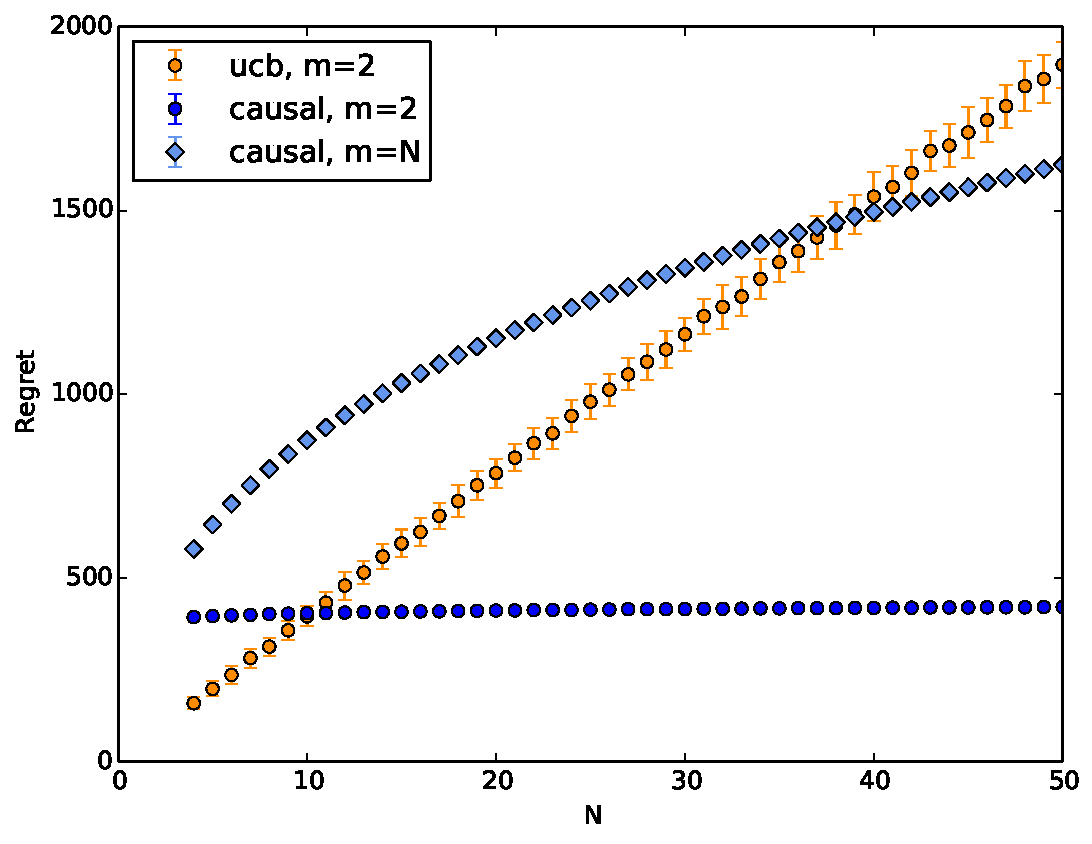
\includegraphics[width=.5\textwidth]{exp_regret_vs_N_T10000_sims100_20151229_113550.pdf}
\end{figure}

\begin{figure}
\caption{Cumulative regret over time for $N = 17$ for UCB with $\alpha=2$, Causal-Explore-Exploit with $m=2$ and Causal-Explore-Exploit with $m=N$. Shaded region shows standard deviation over 100 simulations. The Causal-Explore-Exploit algorithm incurs linear regret during the exploration phase, after which it selects the optimal arm with high probability. For $m=2$, we have $K \sim m^{2/3}T^{1/3}$ and see that we are in the regime in which Causal-Explore-Exploit outperforms UCB.}
\label{fig:known_q_r_vs_t}
\centering
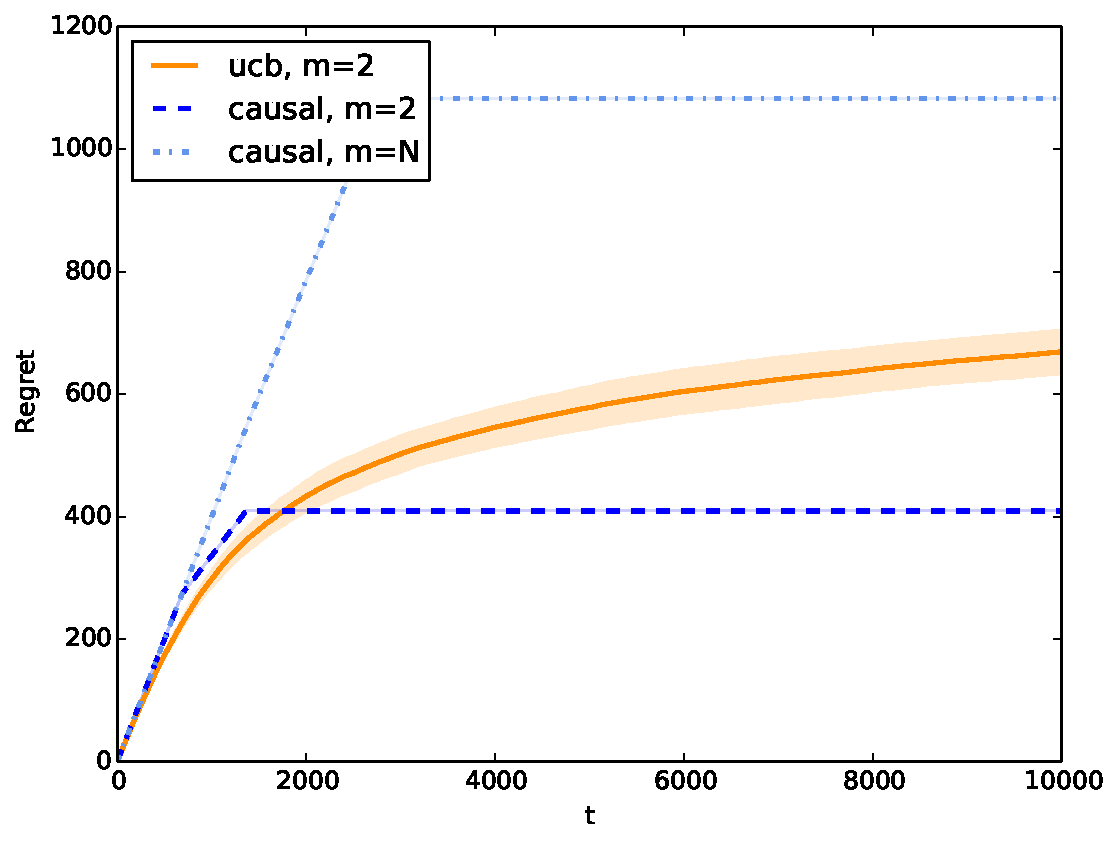
\includegraphics[width=.5\textwidth]{exp_regret_vs_t_T10000_N17_sims100_20151229_120647.pdf}
\end{figure}

\begin{figure}
\caption{Simple regret vs horizon, $T$, for $N = 30$ for UCB with $\alpha=2$, Causal-Best-Arm-Identification with $m=2$ and Causal-Best-Arm-Identification with $m=N$. Error bars show estimated 95\% confidence interval from 1000 simulations.}
\label{fig:simple_vs_T}
\centering
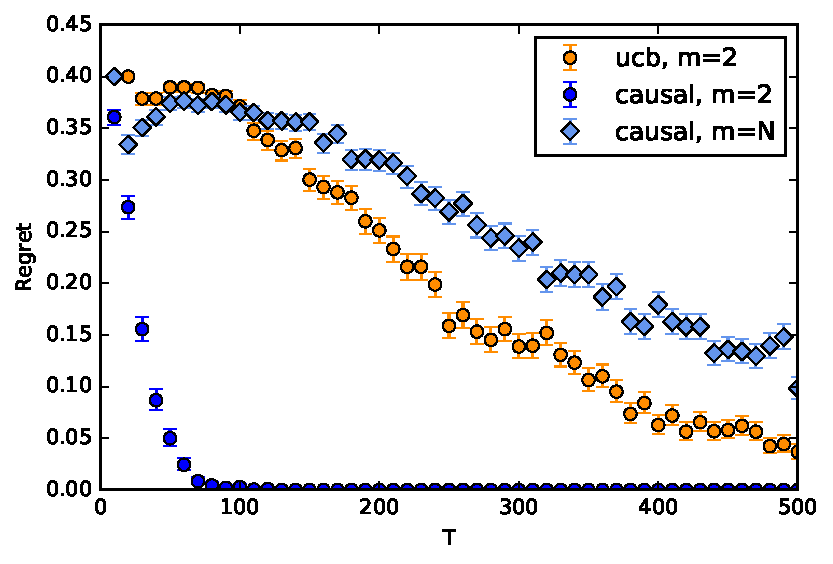
\includegraphics[width=.5\textwidth]{exp_simpleregret_vs_T_N30_sims1000_20160113_010512.pdf}
\end{figure}

\begin{figure}
\caption{Simple regret vs number of variables, $N$, for $T=500$, for UCB with $\alpha=2$, Causal-Best-Arm-Identification with $m=2$ and Causal-Best-Arm-Identification with $m=N$. Error bars show estimated 95\% confidence interval from 1000 simulations.}
\label{fig:simple_vs_N}
\centering
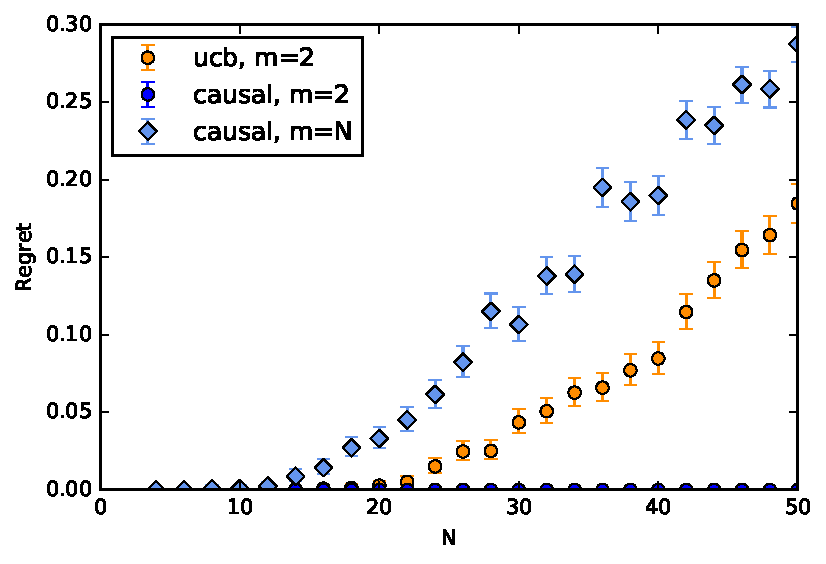
\includegraphics[width=.5\textwidth]{exp_simpleregret_vs_N_T500_sims1000_20160113_010511.pdf}
\end{figure}
%%%%%%%%%%%%%%%%%%%%%%%%%%%%%%%%%%%%%%%%%%%%%%%%%
% DISCUSSION
%%%%%%%%%%%%%%%%%%%%%%%%%%%%%%%%%%%%%%%%%%%%%%%%%
\section{Discussion}


In our algorithm, we have only used the side information provided by the $do()$ action about other actions. Since the $do()$ action fully reveals the value of alternate actions we could have incorporated this information via the graph feedback model \cite{Mannor2011}, where at each timestep the feedback graph $G_t$ is selected stochastically, dependent on $\boldsymbol{q}$, and revealed after an action has been chosen. The feedback graph is distinct from the causal graph. A link $A \rightarrow B$ in $G_t$ indicates that selecting the action $A$ reveals the reward for action $B$. For this specific problem, $G_t$ will always be a star graph with the action $do()$ connected to half the remaining actions. The Exp3-IX algorithm \cite{Kocak2014} was developed for the adversarial version of this problem and has regret $\bigo{\sqrt{\bar{\alpha}T}}$, where $\bar{\alpha}$ is the average independence number of $G_t$. In our case $\bar{\alpha} = \frac{N}{2}$ so we again obtain the regret of the standard bandit algorithm. The issue here is that a malicious adversary can select the same graph each time, such that the rewards for half the arms are never revealed by the informative action. This is equivalent to a, nominally, stochastic selection of feedback graph where $\boldsymbol{q} = \boldsymbol{0}$

\cite{Lelarge2012} consider a stochastic version of the graph feedback problem, but with a fixed graph available to the algorithm before it must select an action. In addition, their algorithm is not optimal for all graph structures and fails, in particular, to provide improvements for star like graphs as in our case. \cite{Buccapatnam2014} improve the dependence of the algorithm on the graph structure but still assume the graph is fixed and available to the algorithm before the action is selected. 

More generally, assuming causal structure creates more complex types of side information, such as that shown in equation \ref{eq:estimation_transfer}. In this case, selecting one action does not fully reveal an alternate action but provides some information towards an estimate. The quality of the estimate notably depends not only on the number of times that action was selected. For example, to get a good estimate for $X_1 = 1$ by intervening on $X_2$ requires us to sample both $X_2=0$ and $X_2=1$, in proportions dependent on $q_2$. This more complex side information does not fit within the graph feedback framework.


\section{Future Open Questions}
\begin{itemize}
\item Known but arbitrary structure
\item Learning structure then exploiting
\end{itemize}
\section{Conclusion}

\bibliography{library}
\bibliographystyle{icml2015}
\end{document}
